\documentclass{llncs}

\usepackage{graphicx,array}
\usepackage{amsmath}
\usepackage{amssymb}
\usepackage{amsfonts}
\usepackage{epsfig}
\usepackage{float}
\usepackage{supertabular} % used in B Symbols


%% Keywords for the B method
\newcommand{\MACHINE}{\operatorname{\mathbf{MACHINE}}}
\newcommand{\REFINEMENT}{\operatorname{\mathbf{REFINEMENT}}}
\newcommand{\IMPLEMENTATION}{\operatorname{\mathbf{IMPLEMENTATION}}}
\newcommand{\REFINES}{\operatorname{\mathbf{REFINES}}}
\newcommand{\SEES}{\operatorname{\mathbf{SEES}}}
\newcommand{\INCLUDES}{\operatorname{\mathbf{INCLUDES}}}
\newcommand{\IMPORTS}{\operatorname{\mathbf{IMPORTS}}}
\newcommand{\SETS}{\operatorname{\mathbf{SETS}}}
\newcommand{\CONSTANTS}{\operatorname{\mathbf{CONSTANTS}}}
\newcommand{\PROPERTIES}{\operatorname{\mathbf{PROPERTIES}}}
\newcommand{\CONCRETE}{\operatorname{\mathbf{CONCRETE}}}
\newcommand{\VARIABLES}{\operatorname{\mathbf{VARIABLES}}}
\newcommand{\ASSERTIONS}{\operatorname{\mathbf{ASSERTIONS}}}
\newcommand{\CONCRETEVARIABLES}{\operatorname{\mathbf{CONCRETE\_VARIABLES}}}
\newcommand{\DEFINITIONS}{\operatorname{\mathbf{DEFINITIONS}}}
\newcommand{\VAR}{\operatorname{\mathbf{VAR}}}
\newcommand{\IN}{\operatorname{\mathbf{IN}}}
\newcommand{\INVARIANT}{\operatorname{\mathbf{INVARIANT}}}
\newcommand{\INITIALISATION}{\operatorname{\mathbf{INITIALISATION}}}
\newcommand{\OPERATIONS}{\operatorname{\mathbf{OPERATIONS}}}
\newcommand{\BEGIN}{\operatorname{\mathbf{BEGIN}}}
\newcommand{\END}{\operatorname{\mathbf{END}}}
\newcommand{\PRE}{\operatorname{\mathbf{PRE}}}
\newcommand{\IF}{\operatorname{\mathbf{IF}}}
\newcommand{\THEN}{\operatorname{\mathbf{THEN}}}
\newcommand{\ELSE}{\operatorname{\mathbf{ELSE}}}
\newcommand{\ELSIF}{\operatorname{\mathbf{ELSIF}}}
\newcommand{\ANY}{\operatorname{\mathbf{ANY}}}
\newcommand{\WHERE}{\operatorname{\mathbf{WHERE}}}
\newcommand{\CASE}{\operatorname{\mathbf{CASE}}}
\newcommand{\OF}{\operatorname{\mathbf{OF}}}
\newcommand{\EITHER}{\operatorname{\mathbf{EITHER}}}
\newcommand{\AND}{\operatorname{\mathbf{AND}}}
\newcommand{\OR}{\operatorname{\mathbf{OR}}}
\newcommand{\NOT}{\operatorname{\mathbf{NOT}}}
\newcommand{\WHILE}{\operatorname{\mathbf{WHILE}}}
\newcommand{\DO}{\operatorname{\mathbf{DO}}}
\newcommand{\VARIANT}{\operatorname{\mathbf{VARIANT}}}
\newcommand{\FALSE}{\operatorname{\mathbf{FALSE}}}
\newcommand{\TRUE}{\operatorname{\mathbf{TRUE}}}

%% Commonly used math entities
\newcommand{\pow}{\operatorname{\mathbb{P}}}
\newcommand{\nat}{\operatorname{\mathbb{N}}}
\newcommand{\pfun}{\operatorname{\rightarrow\mkern-22mu+}}
\newcommand{\fset}{\operatorname{\mathbb{F}}}
\newcommand{\dom}{\operatorname{\mbox{dom}}}
\newcommand{\ran}{\operatorname{\mbox{ran}}}
\newcommand{\natone}{\operatorname{\mathbb{N}_1}}
\newcommand{\integer}{\operatorname{\mathbb{Z}}}
\newcommand{\fun}{\operatorname{\rightarrow}}
\newcommand{\domr}{\operatorname{\triangleleft}}
\newcommand{\seq}{\operatorname{\mathbf{seq1}}}
\newcommand{\ovr}{\operatorname{\oplus}}
\newcommand{\BOOL}{\operatorname{\mathbf{BOOL}}}
\newcommand{\pred}{\operatorname{\mathbf{pred}}}
\newcommand{\Bsucc}{\operatorname{\mathbf{succ}}}


%\usepackage{supertabular}

% DEFINITION DES CARACTERES MATHEMATIQUES B
%------------------------------------------
\def\@setmcodes#1#2#3{{\count0=#1 \count1=#3
	\loop \global\mathcode\count0=\count1 \ifnum \count0<#2
	\advance\count0 by1 \advance\count1 by1 \repeat}}

%\@setmcodes{`A}{`Z}{"7441}
%\@setmcodes{`a}{`z}{"7461}

\mathcode`\;="8000 % Makes ; active in math mode
{\catcode`\;=\active \gdef;{\semicolon\;}}
\mathchardef\semicolon="003B
%    Nominal distance from top of paper to top of page
% \topmargin 0 pt
% \textheight 53\baselineskip
% 
% %   Left margin on odd-numbered pages
% \oddsidemargin  0.15 in
% %   Left margin on even-numbered pages
% \evensidemargin 0.35 in
% %   Width of marginal notes.
% \marginparwidth 1 in
% %   Note that \oddsidemargin = \evensidemargin
% \oddsidemargin 0.25 in
% \evensidemargin 0.25 in
% \marginparwidth 0.75 in
% \textwidth 5.875 in % Width of text line.
% 
% \setlength{\parindent}{0pt}
% \setlength{\parskip}{0ex}

% DEFINITION DES FONTS
%---------------------
% The AMS extra symbol fonts are loaded.
% Note: sometimes called euxm10
\font\msx=msam10
% Note: sometimes called euym10
\font\msy=msbm10

\newfam\msxfam \textfont\msxfam=\msx
\newfam\msyfam \textfont\msyfam=\msy

\def\famletter#1{\ifcase #1 0\or 1\or 2\or 3\or 4\or 5\or 6\or 7\or
	8\or 9\or A\or B\or C\or D\or E\or F\fi}

\edef\fx{\famletter\msxfam}
\edef\fy{\famletter\msyfam}

\def\bbold{\fam\msyfam \msy}

% SYMBOLES B
%-----------
% makes a quoted expression in mathematical text
\def\token#1{\hbox{`$#1$'}}
% used for error messages in Z specs
\def\report#1{\hbox{`{\tt #1}'}}

% \@myop makes an operator, with a strut to defeat TeX's vertical adjustment.
\def\@myop#1{\mathop{\mathstrut{#1}}\nolimits}

% This underscore doesn't have the little kern --- you get an italic
% correction anyway in math mode.
\def\_{\leavevmode \vbox{\hrule width0.5em}}

% Save \q as \xq for quantifiers q.
\let\xforall=\forall
\let\xexists=\exists
\let\xlambda=\lambda
\let\xmu=\mu

% \p and \f make arrows with 1 and 2 crossings resp.
\def\p#1{\mathrel{\ooalign{\hfil$\mapstochar\mkern 5mu$\hfil\cr$#1$}}}
\def\f#1{\mathrel{\ooalign{\hfil
	$\mapstochar\mkern 3mu\mapstochar\mkern 5mu$\hfil\cr$#1$}}}

\let\mc=\mathchardef

\def	\pow		{\mbox{${\cal P}$}}
\def	\po1		{\mbox{${\cal P}_1$}}
\let	\cross		\times
\def	\lambda		{\@myop{\xlambda}}
\def	\lnot		{\neg\;}
\def	\land		{\mathrel{\wedge}}
\def	\lor		{\mathrel{\vee}}
\let	\implies	\Rightarrow
\let	\iff		\Leftrightarrow
\def	\forall		{\@myop{\xforall}}
\def	\exists		{\@myop{\xexists}}
\def	\semi		{\mathrel{\comp}}
\def	\ssemi		{\mathbin{\rm ;}}
\let	\ensembleVide	\emptyset
\let	\rel		\leftrightarrow
\def	\dom		{\@myop{\sf dom}}
\def	\ran		{\@myop{\sf ran}}
\def	\id		{\@myop{\sf id}}
\def	\comp		{\mathbin{\raise
			0.6ex\hbox{\oalign{\hfil$\scriptscriptstyle
			\rm o$\hfil\cr\hfil$\scriptscriptstyle\rm 9$\hfil}}}}
\def	\para		{\mbox{$\mid\mid$}}
\mc	\dres		"2\fx43
\mc	\rres		"2\fx42
\def	\ndres		{\mathbin{{\dres} \llap{$-$}}}
\def	\nrres		{\mathbin{{\rres}\llap{$-$}}}
\def	\lover		{\vartriangleleft{ \llap{$-\!\!\!\!-\!$}}}
\def	\rover		{\mathbin{{\rres}\llap{$\!-\!\!\!-$}}}
\let	\fun		\rightarrow
\def	\pfun		{\p\fun}
\def	\pinj		{\p\inj}
\mc	\inj		"3\fx1A
\def	\psurj		{\p\surj}
\mc	\surj		"3\fx10
\def	\bij		{\surj\!\!\!\!\!\!\!\inj}
\def	\nat		{\mbox{${\cal N}$}}
\def	\na1		{\mbox{${\cal N}_1$}}
\def	\num		{\mbox{${\cal Z}$}}
\def	\int		{\mbox{${\cal Z}$}}
\def	\rat		{\mbox{${\cal Q}$}}
\def	\div		{\mathbin{\rm /}}
\def	\mod		{\mathbin{\bf mod}}
\def	\upto		{\mathbin{\ldotp\ldotp}}
\def	\finset		{\mbox{${\cal F}$}}
\def	\finse1		{\mbox{${\cal F}_1$}}
\def	\ffun		{\f\fun}
\def	\finj		{\f\inj}
\def	\seq		{\@myop{\rm seq}}
\def	\cat		{\mathbin{\raise 0.8ex\hbox{$\mathchar"2\fx61$}}}
\def	\sep		{\hspace*{.05in}}

\setcounter{secnumdepth}{0}
\setcounter{tocdepth}{0}

%-------------------%
% Debut du document %
%-------------------%



 



%
\begin{document}

\title{Formal Modelling of a Microcontroller Instruction Set in B}

\hyphenation{se-pa-ra-te}

\author{Val\'{e}rio Medeiros Jr\inst{1}, David D\'{e}harbe\inst{1}}

\institute{Federal University of Rio Grande do Norte, Natal RN 59078-970, Brazil}

\maketitle

\begin{abstract}
  This paper describes an approach to model the functional aspects of
  the instruction set of microcontroller platforms using the notation
  of the B method. The paper presents specifically the case of the Z80 
  platform. This work is a contribution towards the extension of the
  B method to handle developments up to assembly level code.
\end{abstract}
%
%\keywords{Fomal Methods, microcontroller Verification, Hardware}

\section{Introduction}

The B method~\cite{Abrial} supports the construction of safety systems
models by verification of proofs that guarantees its correctness. So,
an initial abstract model of the system requirements is defined and
then it is refined until the implementation model. Development
environments based on the B method also include source code generators
for programming languages, but the result of this translation
cannot be compared by formal means. The paper \cite{Dantas_SBMF08} presented
recently an approach to extend the scope of the B method up to the
assembly level language. One key component of this approach
is to build, within the framework of the B method, formal models of
the instruction set of such assembly languages.

This work gives an overview of the formal modelling of the instruction
set of the Z80 microcontroller~\cite{Z80_manual}\footnote{The
  interested reader in more details is invited to visit our repository
  at: http://code.google.com/p/b2asm.}. Using the responsibility
division mechanism provided by B, auxiliary libraries of basic modules
were developed as part of the construction of microcontroller
model. Such library has many definitions about common concepts used in
the microcontrollers; besides the Z80 model, it is used by two other
microcontrollers models that are under way.

Other possible uses of a formal model of a microcontroller
instruction set include documentation, the construction of simulators,
and be possibly the starting point of a verification effort for the
actual implementation of a Z80 design. Moreover the model of the
instruction set could be instrumented with non-functional aspects,
such as the number of cycles it takes to execute an instruction, to
prove lower and upper bounds on the execution time of a routine. The
goal of this project, though, is to provide a basis for the generation
of software artifacts at the assembly level that are amenable to 
refinement verification within the B method.

This paper is focused on the presentation of the Z80 model, including
elementary libraries to describe hardware aspects. The paper is
structured as follows. Section~\ref{sec:B_method} provides a short
introduction to the B method. Section~\ref{sec:models} presents the
elementary libraries and the modelling of some elements common to
microcontrollers.  Section~\ref{sec:z80} presents the B model of the
Z80 instruction set. Section ~\ref{sec:Proofs} provides some
information on the proof effort needed to analyze the presented
models. Related work is discussed in
Section~\ref{sec:relatedworks}. Finally, the last section is devoted
to the conclusions.

\section{Introduction to the B Method}
\label{sec:B_method}

The B method for software development~\cite{Abrial} is based on the B Abstract
Machine Notation (AMN) and the use of formally proved refinements up to a
specification sufficiently concrete that programming code can be automatically
generated from it. Its mathematical basis consists of first order logic, integer
arithmetic and set theory, and its corresponding constructs are similar to those
of the Z notation.


A B specification is structured in modules. A module defines a set of valid
states, including a set of initial states, and operations that may provoke a
transition between states. The design process starts with a module with a
so-called functional model of the system under development. In this initial
modelling stage, the B method requires that the user proves that, in a machine,
all the its initial states are valid, and that operations do not define
transitions from valid states to invalid states.
  
Essentially, a B module contains two main parts: a header and the available
operations. Figure~\ref{fig:maqB} has a very basic example. The clause
$\mathit{MACHINE}$ has the name of module.  The next two clauses respectively
reference external modules and create an instance of an external module. The
$\mathit{VARIABLES}$ clauses declares the name of the variables that compose the
state of the machine. Next, the $\mathit{INVARIANT}$ clause defines the type and
other restrictions on the variables. The $\mathit{INITIALIZATION} $ specifies
the initial states. Finally, operations correspond to the transitions between
states of the machine.


\begin{figure}
  % \begin{small}
  $$
  \begin{array}{lcl}
    \begin{array}[t]{l}
      \MACHINE \quad  \mathit{micro} \\
      \SEES \quad \mathit{TYPES}, \mathit{ALU} \\
      \INCLUDES  \quad \mathit{MEMORY} \\
      \VARIABLES \quad    \mathit{pc}  \\
      \INVARIANT \quad \mathit{pc} \in \mathit{INSTRUCTION} 
    \end{array}
    & \hspace*{1cm} &
    \begin{array}[t]{l}
      \INITIALISATION  \mathit{pc} := 0 \\
      \OPERATIONS\\
      \mathit{JMP} \mathit{( jump )} = \\
      \quad \PRE \mathit{jump} \in \mathit{INSTRUCTION}\\ 
      \quad \THEN \mathit{pc} := \mathit{jump}\\  
      \quad \END \\
      \END
    \end{array}
  \end{array}
  $$
\caption{A very basic B machine.}
\label{fig:maqB}
\end{figure}


\section{Model structure and basic components}
\label{sec:models}

We have been developed a reusable set of basic definitions to model
hardware concepts and data types concepts. These definitions are
grouped into two separate development projects and are available as
libraries. A third project is devoted to the higher-level aspects of
the platform. Thus, the workspace is composed of: a hardware library,
a types library and a project for the specific platform, in this case
the Z80. The corresponding dependency diagram is depicted in
Figure~\ref{fig:hardware-definition-graph}; information specific to
each project is presented in the following.

\begin{figure}[h] \centering
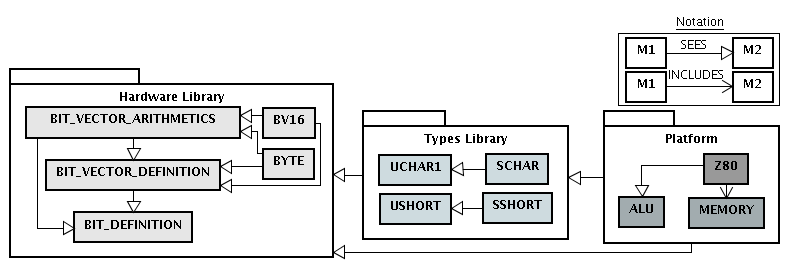
\includegraphics[width=.92\textwidth]{diagramaEstrutural.png}
 \caption{Dependency diagram of the Z80 model.}
\label{fig:hardware-definition-graph}
\end{figure}



\subsection{Bit Representation and Manipulation}

The entities defined in the module $\mathit{BIT\_DEFINITION}$ are the
type for bits, logical operations on bits (negation, conjunction,
disjunction, exclusive disjunction), as well as a conversion function
from booleans to bits.

First, bits are modelled as a set of integers: $\mathit{BIT} =
\mathit{0..1}$. The negation is an unary function on bits and it is
defined as:

$
\begin{array}{l}
\mathit{bit\_not}  \in  \mathit{BIT}  \fun  \mathit{BIT}  \land \forall ( \mathit{bb}). (\mathit{bb} \in \mathit{BIT} \implies \mathit{bit\_not}(\mathit{bb}) =
1-\mathit{bb})\\
\end{array}
$

The module also provides lemmas on negation that may be useful for the
users of the library to develop proofs:

$
\begin{array}{l}
%  \mathit{bit\_not}(0) = 1;  \mathit{bit\_not}(1) = 0; \\
\forall (\mathit{bb}).(\mathit{bb} \in \mathit{BIT} \implies \mathit{bit\_not}(\mathit{bit\_not}(\mathit{bb})) = \mathit{bb})
\end{array}
$

Conjunction is an unary function on bits and it is defined as:

$
\begin{array}{l}
\mathit{bit\_and} \in \mathit{BIT} \times \mathit{BIT} \fun \mathit{BIT} \land \\
\forall (\mathit{b1}, \mathit{b2}).(\mathit{b1}  \in \mathit{BIT}  \land \mathit{b2} \in \mathit{BIT} \implies \\
\quad ((\mathit{bit\_and}(\mathit{b1}, \mathit{b2}) = 1) \iff (\mathit{b1} = 1)  \land  (\mathit{b2} = 1)))
\end{array}
$

The module provides the following lemmas for conjunction, either:

$
\begin{array}{l}
%  \mathit{bit\_and}(0,0) = 0;  \mathit{bit\_and}(0,1) = 0; \\
%  \mathit{bit\_and}(1,0) = 0;  \mathit{bit\_and}(1,1) = 1; \\
\forall (\mathit{b1},\mathit{b2}).(\mathit{b1} \in \mathit{BIT} \land \mathit{b2} \in \mathit{BIT} \implies \\
\quad (\mathit{bit\_and}(\mathit{b1}, \mathit{b2}) = \mathit{bit\_and}(\mathit{b2},\mathit{b1})))\land \\
\forall (\mathit{b1},\mathit{b2},\mathit{b3}).(\mathit{b1} \in \mathit{BIT} \land  \mathit{b2} \in \mathit{BIT} \land \mathit{b3} \in \mathit{BIT} \implies \\
\quad (\mathit{bit\_and}(\mathit{b1}, \mathit{bit\_and}(\mathit{b2},\mathit{b3})) = \mathit{bit\_and}(\mathit{bit\_and}(\mathit{b1},\mathit{b2}),\mathit{b3})))\\
% \forall (\mathit{b1}).(\mathit{b1} \in \mathit{BIT} \implies (\mathit{bit\_and}(\mathit{b1}, 1) = \mathit{b1})); \\
% \forall (\mathit{b1}).(\mathit{b1} \in \mathit{BIT} \implies (\mathit{bit\_and}(\mathit{b1}, 0) = 0));
\end{array}
$

The module provides definitions of $\mathit{bit\_or}$ (disjunction)
and $\mathit{bit\_xor}$ (exclusive disjunction), as well as lemmas on
those operators. These are standard and their expression in B is
similar as for $\mathit{bit\_and}$, they are thus omitted.

Finally, the conversion from booleans to bits is simply defined as:

$
\begin{array}{l}
\mathit{bool\_to\_bit} \in \BOOL \fun \mathit{BIT} \land \mathit{bool\_to\_bit} = \{ \TRUE \mapsto 1, \FALSE \mapsto 0 \} \\
\end{array}
$

Observe that all the lemmas that are provided in this module have been
mechanically proved by the theorem prover included with our B
development environment. None of these proofs requires human insight.


\subsection{Representation and Manipulation of Bit Vectors}

Sequences are pre-defined in B, as functions whose the domain is an
integer range with lower bound 1 (one). Indices in bit vectors usually
range from 0 (zero) upwards and the model we propose obeys this
convention by making an one-position shift where necessary. This shift
is important to use the predefined functions of sequences. We thus
define bit vectors as non-empty sequences of bits, and
$\mathit{BIT\_VECTOR}$ is the set of all such sequences: 
$\mathit{BIT\_VECTOR} = \seq (\mathit{BIT})$.

The function $\mathit{bv\_size}$ returns the size of a given bit vector. It is basically a wrapper for the
predefined function $\mathbf{size}$ that applies to sequences.

$
\begin{array}{l}
\mathit{bv\_size} \in \mathit{BIT\_VECTOR} \fun \nat_1 \land \\
\mathit{bv\_size} = \lambda bv . (bv \in \mathit{BIT\_VECTOR} \mid \mathbf{size}(bv))
\end{array}
$

We also define two functions $\mathit{bv\_set}$ and $\mathit{bv\_clear}$ that, given a bit vector, and a position of
the bit vector, return the bit vector resulting from setting the corresponding position to 0 or to 1, and a function
$\mathit{bv\_get}$ that, given a bit vector, and a valid position, each one returns the value of the bit at that
position. Only the first definition is shown here:

$
\begin{array}{l}
\mathit{bv\_set} \in \mathit{BIT\_VECTOR} \times \nat \fun \mathit{BIT\_VECTOR} \land \mathit{bv\_set} =\\
\lambda v, n . (v \in \mathit{BIT\_VECTOR} \land n \in \nat \land n <\mathit{bv\_size}(v)
\mid v \lover \{ n+1 \mapsto 1 \})
\end{array}
$


Additionally, the module provides definitions for the classical
logical combinations of bit vectors: $\mathit{bit\_not}$,
$\mathit{bit\_and}$, $\mathit{bit\_or}$ and $\mathit{bit\_xor}$. Only
the first two are presented here. Observe that the domain of the
binary operators is restricted to pairs of bit vectors of the same
length:

$
\begin{array}{l}
\mathit{bv\_not} \in \mathit{BIT\_VECTOR} \fun \mathit{BIT\_VECTOR} \land \\
\mathit{bv\_not} = \lambda v . (v \in \mathit{BIT\_VECTOR} \mid \quad \lambda i . (1 .. \mathit{bv\_size}(v)) \mid \mathit{bit\_not}(v(i))) \land \\
\mathit{bv\_and} \in \mathit{BIT\_VECTOR} \times \mathit{BIT\_VECTOR} \fun \mathit{BIT\_VECTOR} \land \\
\mathit{bv\_and} = \lambda v_1, v_2 . (v_1 \in \mathit{BIT\_VECTOR} \land v_2 \in \mathit{BIT\_VECTOR} \land \\
\quad \mathit{bv\_size}(v_1) = \mathit{bv\_size}(v_2) \mid \lambda i . (1 .. \mathit{bv\_size}(v_1)) \mid
\mathit{bit\_and}(v_1(i), v_2(i)))
\end{array}
$

We provide several lemmas on bit vector operations. These lemmas
express properties on the size of the result of the operations
as well as classical algebraic properties such as associativity
and commutativity.
 
\subsection{Modelling Bytes and Bit Vectors of Length 16}

Bit vectors of length 8 are bytes. They form a common entity in
hardware design. We provide the following definitions:


\hspace*{0.0in}\it BYTE\_WIDTH \rm = 8 $\land$ \it BYTE\_INDEX \rm = 1 $\upto$ \rm  BYTE\_WIDTH\rm $\land$

\hspace*{0.0in}\it PHYS\_BYTE\_INDEX \rm = \rm 0 $\upto$ \rm (\it BYTE\_WIDTH\rm -\rm 1\rm )\hspace*{0.10in} $\land$ 

\hspace*{0.0in}\it BYTE \rm = \rm \{ \it bt  $\mid$  \it bt $\in$ \it BIT\_VECTOR  $\land$  \it bv\_size\rm (\it bt\rm )\rm =\it BYTE\_WIDTH\rm \}\hspace*{0.10in} $\land$ 

\hspace*{0.0in}\it BYTE\_ZERO  $\in$  \it BYTE  $\land$ \it BYTE\_ZERO \rm = \it BYTE\_INDEX  $\times$  \rm \{\rm 0\rm \}

The $\mathit{BYTE\_INDEX}$ is the domain of the functions modelling bytes. It
starts at 1 to obey a definition of sequences from B. However, it is common in
hardware architectures to start indexing from zero. The definition
$\mathit{PHYS\_BYTE\_INDEX}$ is used to provide functionalities obeying this
convention. The $\mathit{BYTE}$ type is a specialized type from
$\mathit{BIT\_VECTOR}$, but it has a size limit. Other specific definitions are
provided to facilitate further modelling: the type $\mathit{BV16}$ is created for
bit vector of length 16 in a similar way.


\subsection{Bit Vector Arithmetics}

Bit vectors are used to represent and combine numbers: integer ranges
(signed or unsigned). Therefore, our library includes functions to
manipulate such data, for example, the function $\mathit{bv\_to\_nat}$
that maps bit vectors to natural numbers:


$
\begin{array}{l}
\mathit{bv\_to\_nat} \in \mathit{BIT\_VECTOR} \fun \nat \land \\
\mathit{bv\_to\_nat} = \lambda v . (v \in \mathit{BIT\_VECTOR} \mid \sum i . (i \in \dom(v) . v(i)
\times 2^{i-1}))
\end{array}
$

An  associated lemma is: $\forall n . (n \in \nat_1 \implies \mathit{bv\_to\_nat}(\mathit{nat\_to\_bv}(n)) = n)$

\subsection{Basics Data Types}

The instruction set of microcontrollers usually have common data
types. These types are placed in the types library. Each type module
has functions to manipulate and convert its data. There are six common
basics data types represented by modules, see details in
table~\ref{tab:types}.

\begin{table}
\caption{Descriptions of basic data types}
\label{tab:types}

\begin{center}
\begin{tabular}{|c|c|c|c|c|c|c|}
\hline
 $Type\ Name$ & UCHAR & SCHAR & USHORTINT & SSHORTINT  & BYTE & BV16 \\\hline
 $Range$ & 0..255 & -128..127 & 0..65.535  & -32.768..32.767  & -- & --\\ \hline
 $Physical\ Size $ & 1 byte & 1 byte & 2 bytes & 2 bytes &  1 bytes & 2 bytes \\ \hline
\end{tabular}
\end{center} 
\end{table}

Usually, each type module just needs to instantiate concepts that were
already defined in the hardware modelling library.  For example, the
function $\mathit{bv\_to\_nat}$ from bit vector arithmetics is
specialized to $\mathit{byte\_uchar}$. As the set $\mathit{BYTE}$ is a
subset of the $\mathit{BIT\_VECTOR}$, this function can defined
as follows:

$
\begin{array}{l}
\mathit{byte\_uchar} \in \mathit{BYTE} \fun \nat \land \\
\mathit{byte\_uchar} = \lambda (v) . ( v \in BYTE | bv\_to\_nat(v) )
\end{array}
$

The definitions of the library types reuse the basic definitions from
the hardware library. This provides greater confidence and facilitates
the proof process, because the prover can reuse the previously defined
lemma.

The inverse function $\mathit{uchar\_byte}$ is easily defined:

$
\begin{array}{l}
\mathit{uchar\_byte} \in \mathit{UCHAR}  \fun  \mathit{BYTE}  \land \\
   \mathit{uchar\_byte} = \ (\mathit{byte\_uchar}) ^{-1}
\end{array}
$ 

% We also created the following lemmas:
%  
% $
% \begin{array}{l}
%  \forall (val) . (val \in \mathit{UCHAR} |
%  \mathit{byte\_uchar}(\mathit{uchar\_byte}(val)) = val) \land\\
%  \forall (by) . (by \in \mathit{BYTE} |
%  \mathit{uchar\_byte}(\mathit{byte\_uchar}(by)) = by)
% \end{array}
% $ 

Similarly, several other functions and lemmas were created for all other
data types.

\section{Description of the Z80 B model }
\label{sec:z80}

The \textit{Z80} is a CISC microcontroller developed by
\textit{Zilog}~\cite{Z80_manual}. It supports 158 different instructions and all
of them were specified. These instructions are classified into these categories:
load and exchange; block transfer and search; arithmetic and logical; rotate and
shift; bit manipulation; jump, call and return; input/output; and basic cpu
control.


The main module includes an instance of the memory module and accesses the
definitions from basic data types modules and the \textit{ALU} module.

\begin{sloppypar}

\bf MACHINE

\hspace*{0.15in}\it Z80

\bf INCLUDES

\hspace*{0.10in}\it MEMORY

\bf SEES

\hspace*{0.10in}\it ALU, \it BIT\_DEFINITION, \it BIT\_VECTOR\_DEFINITION,

\hspace*{0.10in}\it BYTE\_DEFINITION, \it BV16\_DEFINITION, 

\hspace*{0.10in}\it UCHAR\_DEFINITION, \it SCHAR\_DEFINITION,

\hspace*{0.10in}\it SSHORT\_DEFINITION ,\it USHORT\_DEFINITION
\end{sloppypar}

% Chacteristics of microcontroller
Each instruction is represented by a B operation in the module Z80. By
default, all parameters from operations are either predefined elements
in the model or integers values in the decimal representation.  The
internal registers contain 208 bits of reading/writing memory. It
includes two sets of six general purpose registers which may be used
individually as 8-bits registers or as 16-bits register pairs.  The
working registers are represented by variable $\mathit{rgs8}$. The
domain of $\mathit{rgs8}$ ($\mathit{id\_regs8}$) is a set formed by
identifiers of registers of 8 bits. These registers can be accessed in
pairs, forming 16-bits, resulting in another set of identifiers of
16-bits registers, named $\mathit{id\_reg16}$. The main working
register of Z80 is the accumulator ($\mathit{rgs8(a0)}$) used for
arithmetic, logic, input/output and loading/storing operations.

\subsection{Modelling Registers, Input and Output Ports and Instructions}

The Z80 has different types of registers and instructions. The CPU
contains general-purpose registers ($\mathit{id\_reg\_8}$), a stack
pointer ($\mathit{sp}$), program counter ($\mathit{pc}$), two index
registers ($\mathit{ix}$ and $\mathit{iy}$), an interrupt register
($\mathit{i\_}$), a refresh register ($\mathit{r\_}$), two bits
($\mathit{iff1}$, $\mathit{iff2}$) used to control the interruptions,
a pair of bits to define the interruption mode ($\mathit{im}$) and the
input and output ports ($\mathit{i\_o\_ports}$). Below, part of the
corresponding definitions are replicated from the $\INVARIANT$:
   
\begin{sloppypar}
%\bf INVARIANT
\hspace*{0.10in}\it rgs8  $\in$  \it id\_reg\_8  $\fun$  \it BYTE  $\land$ pc  $\in$  \it INSTRUCTION  $\land$ 

\hspace*{0.10in}\it  sp  $\in$  \it BV16  $\land$  \it ix  $\in$  \it BV16  $\land$  \it iy  $\in$  \it BV16  $\land$ 

\hspace*{0.10in}\it i\_  $\in$  \it BYTE  $\land$  \it r\_ $\in$  \it BYTE  $\land$ iff1  $\in$  \it BIT
$\land$ \it iff2  $\in$  \it BIT  $\land$ 

\hspace*{0.10in}\it im \rm $\in$ \rm (\it BIT $\times$ \it BIT\rm )  $\land$ i\_o\_ports  $\in$  \it BYTE 
$\fun$  \it BYTE
\end{sloppypar}

A simple example of instruction is a $\mathit{LD\_n\_A}$, as shown
below.  Many times, to model an instruction is necessary to use the
predefined functions, these help the construction of model. This
instruction use the $\mathit{updateAddressMem}$ function from
\textit{Memory} module and it receives an address memory and its new
memory value. Finally it increments the program counter
($\mathit{pc}$) and update the refresh register ($\mathit{r\_}$).
	
\hspace*{0.00in}\bf LD\_n\_A \rm ( \it nn \rm ) \rm =
	
\hspace*{0.20in}\bf PRE \it nn $\in$ \it USHORT\hspace*{0.15in} %$\land$  \it nn $\in$\it DATA\_R\_ADR
	
\hspace*{0.20in}\bf THEN
	
\hspace*{0.20in}\bf updateAddressMem \rm ( \it ushort\_to\_bv16 \rm ( \it nn \rm ) \rm , \it rgs8 \rm ( \it a0 \rm )
\rm )  $\para$
	
\hspace*{0.20in}\it pc \rm := \it instruction\_next \rm ( \it pc \rm )  $\para$  \it r\_ \rm := \it
update\_refresh\_reg\rm (\it r\_\rm )
	
\hspace*{0.00in}\bf END\rm 
	
The microcontroller model can specify security properties. For example, the
last operation could have a restriction to write only in a defined region of memory.


\section{Proofs}
\label{sec:Proofs}
% [O que as provas garantem? citar que dificeis, que � necess�rio buscar t�cnicas eficientes
% para realizar as provas ]

The proof obligations allow to verify the data types, important system
properties and if the expressions are well-defined (WD)\footnote{An
  expression is called ``well-defined'' (or unambiguous) if its
  definition assigns it a unique interpretation or value.}. The
properties provide additional guarantees, because they can set many
safety rules. However, the model can be very difficult to prove.
 
% [Conclusao] This project has many proof obligations and
% The construction of then model was a difficult task, as several
% iterations were needed to provide the good library definitions 
% as well as to optimize the definition of the functionality of
% the microprocessor instructions by grouping common data
% manipulation into auxiliary functions.

Several iterations were needed to provide the good library definitions as well as
to fine-tune the model of the microcontroller instructions by factoring common
functionalities into auxiliary definitions.




However, few proof commands\footnote{The proof commands are steps that direct the
prover to find the proof, and cannot introduce false hypothesis.} need to be used
to prove most proof obligations. As there are many similar assembly instructions,
some human-directed proofs, when replayed, could discharge other proof
obligations. A good example is a set of 17 proof commands that quickly aided the
verification of 99\% (2295) of WD proofs. We also set up a proving environment
consisting of networked computers to take advantage of the distribution
facilities now provided in the B development environment. Finally, all of the
2926 proof obligations were proved using the tool support of the development
environment.
 
\section{Related Works}
\label{sec:relatedworks}
 
There are in the literature of computer science some
approaches~\cite{BHDL_2003,GEMPLUS_99} to model hardware and the virtual machines
using the B method. Then, in both works the B method has been used successfully
to model the operational semantic. However the cost of modelling was still expensive and this
paper quoted some techniques to lower the cost of modelling.
% Although, the modelling of the Z80 do not have modelled some small aspects.


% The objective of researchers


In general, the researchers employing the B method have focused on
more abstract level of description of software.  Considering low-level
aspect, there has been previous work on modelling the Java Virtual
Machine~\cite{GEMPLUS_99}.

The main motivation of our research is the development of verified
software up to the assembly level, which requires specifying the
semantics of the underlying hardware. Thus, some aspects were not
modelled in our work such as the execution time of the instructions.
Also we did not consider the microarchitecture of the hardware as the scope of
our work does not include hardware verification. However, there are
many other specialized techniques to verify these questions.
 
 \section{Conclusions}
\label{sec:conclusions} 

This work has shown an approach to the formal modelling of the instruction set of
microcontrollers using the B method. During the construction of this model, some
ambiguities and errors were encountered in the official reference for Z80
microcontroller~\cite{Z80_manual}. As the B notation has a syntax that is not too
distant from that of imperative programming languages, such model could be used
to improve the documentation used by assembler programmers. Besides, the formal
notation used is analyzed by software that guarantees the correctness of typing,
the well-definedness of expressions, in addition to safety properties of the
microcontroller state.


% This research is much interesting to
% design microcontroller. Because, the building of formal model found some erros and ambiguities at the oficial
% manual~\cite{Z80_manual}. The Z80's B model can replace the documentation used by assembler programmers, because the
% formal model represents the instructions effects and the B-method has a easy language, that remembers the pascal
% language. Besides, the formal model restricts the defintions to correct typing, use expressions well-defined and
% allow to verify properties on the model.


% [Trabalhos futuros ]
Future works comprise the development of software with the B method
from functional specification to assembly level, using the Z80 model
presented in this paper. The mechanic compilation from B algorithmic 
constructs to assembly platform is also envisioned.

%  The next steps of the work comprises the development of a real study case in the oil area and the project of a
% compiler to aid the automatization of verification at the assembly level
 
% The next works are the development of a real study case in the oil area and after the project of a compiler to aid
% the automatization of verification at the assembler level.
  
\paragraph{Acknowledges:}
This work received support from ANP (\textit{Ag\^{e}ncia Nacional do
  Petr\'{o}leo, G\'{a}s Natural e Biocombust\'{\i}veis}) and CNPq
(\textit{Conselho Nacional de Desenvolvimento Cient\'{\i}fico e
  Tecnol\'{o}gico}).

\begin{thebibliography}{5}

\bibitem {Abrial}
Abrial, J. R. The B Book: Assigning Programs to Meanings. Cambridge University Press, United States of
America, 1 edition, 1996.

\bibitem {BHDL_2003}    
Aljer, P. Devienne; S. Tison  J-L. Boulanger and G. Mariano. Bhdl: Circuit Design in B. A. In
ACSD, Third International Conference on Application of Concurrency to System Design, pages 241-242, 2003.

\bibitem {GEMPLUS_99}
Casset L.; Lanet J. L. A Formal Specification of the Java Bytecode Semantics using the B
method.Technical Report, Gemplus. 1999.

% \bibitem {CLEARSY}
% Clearsy. Atelier B. http://www.atelierb.eu.

\bibitem {Dantas_SBMF08}
Dantas, B; D\'{e}harbe, D.; Galv\~{a}o, S. L.; Moreira, A. M. and
Medeiros Jr, V. G.. Applying the B Method to Take on the Grand Challenge of
Verified Compilation. In: SBMF, Savaldor, 2008. SBC.
 
\bibitem {HOARE}
Hoare, C. A. R. The verifying compiler, a grand challenge for computing research.
In: VMCAI, p. 78-78, 2005.


\bibitem{Z80_manual}
Zilog. Z80 Family CPU User Manual. http://www.zilog.com/docs/z80/um0080.pdf

\end{thebibliography}

\end{document}
%
% \bibitem {clar:eke}
% Clarke, F., Ekeland, I.:
% Nonlinear oscillations and
% boundary-value problems for Hamiltonian systems.
% Arch. Rat. Mech. Anal. {\bf 78} (1982) 315--333
% %
% \bibitem {clar:eke:2}
% Clarke, F., Ekeland, I.:
% Solutions p\'{e}riodiques, du
% p\'{e}riode donn\'{e}e, des \'{e}quations hamiltoniennes.
% Note CRAS Paris {\bf 287} (1978) 1013--1015
% %
% \bibitem {mich:tar}
% Michalek, R., Tarantello, G.:
% Subharmonic solutions with prescribed minimal
% period for nonautonomous Hamiltonian systems.
% J. Diff. Eq. {\bf 72} (1988) 28--55
% %
% \bibitem {tar}
% Tarantello, G.:
% Subharmonic solutions for Hamiltonian
% systems via a $\bbbz_{p}$ pseudoindex theory.
% Annali di Matematica Pura (to appear)
% %
% \bibitem {rab}
% Rabinowitz, P.:
% On subharmonic solutions of a Hamiltonian system.
% Comm. Pure Appl. Math. {\bf 33} (1980) 609--633
% \end{thebibliography}
%

